\begin{frame}[fragile]{TAMD predicts HIV-1 gp120 conformational changes}
\begin{tikzpicture}
\pcuad{\textwidth}{\textheight}
\path(nw) ++(-0.75,0.0) node(text)[anchor=north west,text width=\textwidth]{{\tiny \textcolor{red!80!black}{CFA and E. Vanden-Eijnden {\it PNAS} {\bf 107}:4961 (2010).}}} ++(0,-0.33) node(topfig)[graphics,anchor=north west]{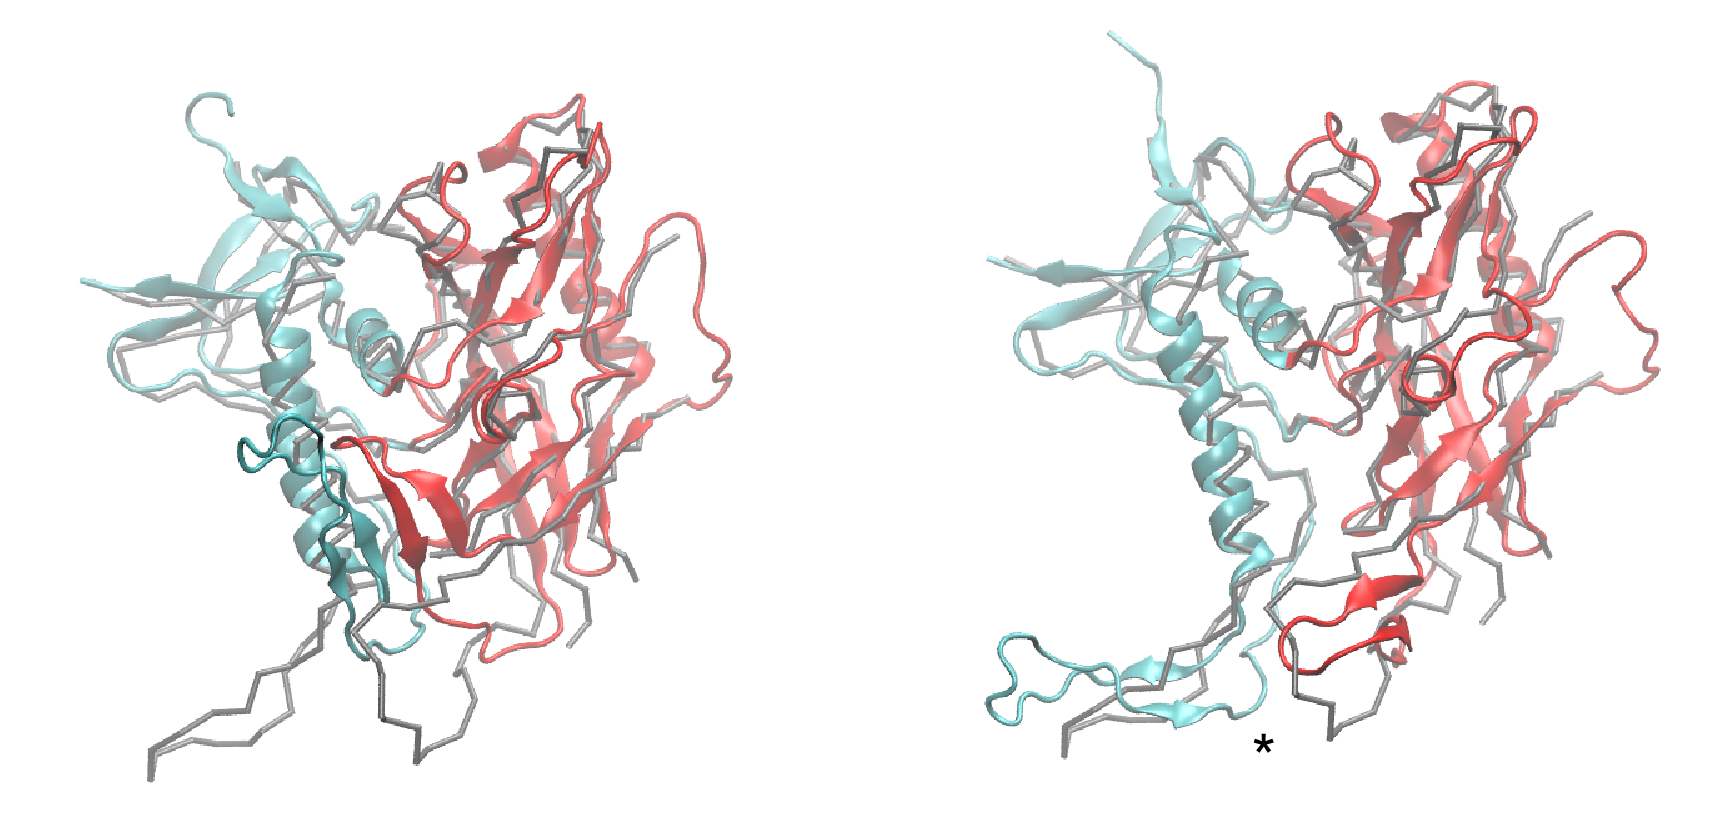
\includegraphics[width=0.8\textwidth]{gp120_snap.png}} ++(0,-4) node(botfig)[graphics,anchor=north west]{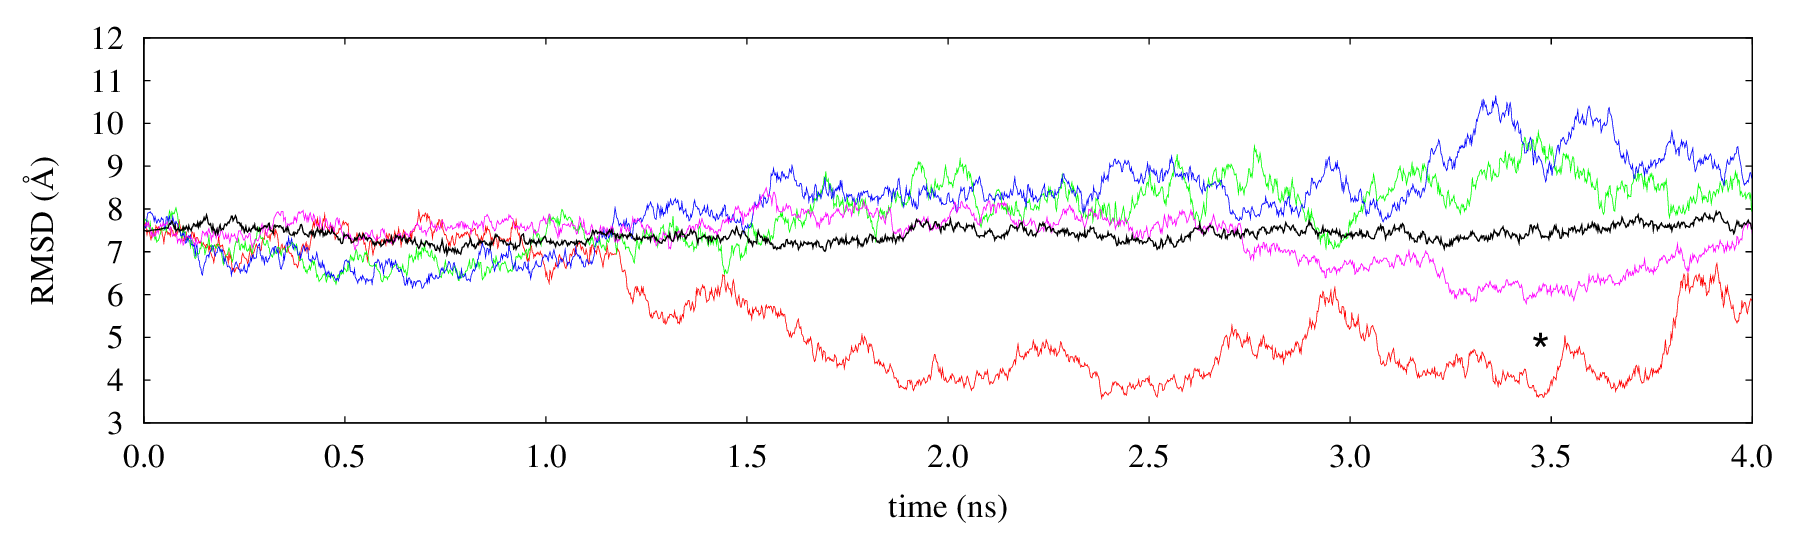
\includegraphics[width=\textwidth]{gp120_rmsdplot.png}}; 
\path(ne) ++(0,0) node(text2)[anchor=north east,text width=0.3\textwidth]{
\begin{itemize}
\item Ribbon: TAMD from 1GC1 (ground state) (\textcolor{teal}{inner}/\textcolor{red}{outer})
\item Tube: Reference from 3HI1 (Ab-F105-bound)
\end{itemize}};
\end{tikzpicture}
\end{frame}

